\section{Experiments}
\label{sec:experiments}
Errors are RMSE in standardised units over the targets of a held-out model, with 95\% bootstrap intervals over held-out models (Section~\ref{sec:setting}); on MTEB-A1 and A2 each cell is the mean of 10 repetitions of 5-fold splits, and random selection averages at least 100 draws.
Inference is the factor posterior unless stated; the matrices are listed in Table~\ref{tab:t1} (Appendix~\ref{app:data}).
The selectors are the A-optimal criterion on the latent factors (the declared one) and the complement-error greedy$^\dagger$, added after a pilot on a separate seed had shown the A-optimal criterion degrading at large $k$.


\subsection{How fast the error falls with $k$}
Figure~\ref{fig:f1} answers the question on the complete MTEB block A1.
With no benchmark run, the history-mean predictor has RMSE $1.03$.
Running three of the 202 benchmarks, chosen by the A-optimal criterion, brings it to $0.595$ [0.554, 0.637], against $0.701$ [0.657, 0.742] for three random ones; the gain over random is $28\%$ in MSE at $k=3$, $15\%$ at $k=8$ and $3\%$ at $k=20$ (Table~\ref{tab:t2}, all Holm-significant).
After the first few benchmarks the curve flattens: from $k=8$ to $k=20$ the best selector moves from $0.55$ to $0.49$, and an RMSE of $0.5$ is reached at $k=20$ by the complement-error greedy, at $k=60$ by random choice, and never by the A-optimal criterion, whose error rises again after $k\approx15$.
With ExtraTrees inference both selections are lower at small $k$ and the gap between them narrows to $0.017$ in RMSE at $k=8$ ($0.506$ against $0.523$) and $0.011$ at $k=12$ (dashed curves): the advantage of selection does not depend on the factor model, but beyond $k\approx10$ it is small on A1 under any imputer.
The decision metrics move more slowly: for the complement-error greedy the pairwise accuracy of ``which history models does the new model beat'' is $0.856$ at $k=3$ and $0.899$ at $k=60$ (random: $0.828$, $0.882$), and the top-10 F1 $0.61$ and $0.74$.

\subsection{Does the theory predict the curve?}
Figure~\ref{fig:f2} separates the two questions.
Where the truth is known (synthetic matrices with $N=48$, three spectra, $M\in\{30,60,125,500\}$, three signal-to-noise levels, 252 cells), the closed form of Proposition~\ref{prop:decomp} with the true parameters stays within 10\% of the measured error in 97\% of cells (median gap 1.8\%), meeting the pre-declared threshold of 90\%.
With parameters fitted from $M$ models it does not: the plug-in forecast stays within 10\% in 72\% of cells and the finite-history forecast in 73\%, so the correction of Section~\ref{sec:theory} does not improve on the plug-in; both fail the threshold at $M=30$ and $M=60$ (27\%, and 62\% and 65\% of cells within 10\%) and pass it at $M\ge125$ (98--100\%).
The effective-rank prediction of Conjecture~\ref{conj:fm} holds in 27 of 36 cells (rank chosen by held-out likelihood within 2 of $r_{\rm eff}(M)$); eight of the nine misses are the power-law spectrum with $M<500$, so we read the conjecture as supported for block spectra and an over-estimate for slowly decaying ones.

On the real matrices the forecast built from the history fit alone is optimistic.
On A1 its signed error in RMSE is $-10\%$ at $k=1$ and $-19\%$ at $k=20$, on A2 $-6\%$ and $-20\%$; the median gap is $15\%$ (A1) and $11\%$ (A2), within the 20\% tolerance we had set for real matrices and outside the 10\% we had set for synthetic ones from $k=3$ on.
The rank chosen by held-out likelihood is within 2 of the predicted effective rank in every fold (A1: 8.3 against 8.3; A2: 4.8 against 4.7).
Varying the history size shows where this stops holding: the forecast is optimistic at every $M$ on MTEB and the rank is resolved only when the history is nearly the whole matrix, whereas on the Open LLM Leaderboard matrices ($M$ up to $2000$) the gap is at most $3.4\%$ from $M=500$; the correction helps when $M$ is large against $N$ (Appendix~\ref{app:history}).

\begin{figure}[t]
\centering
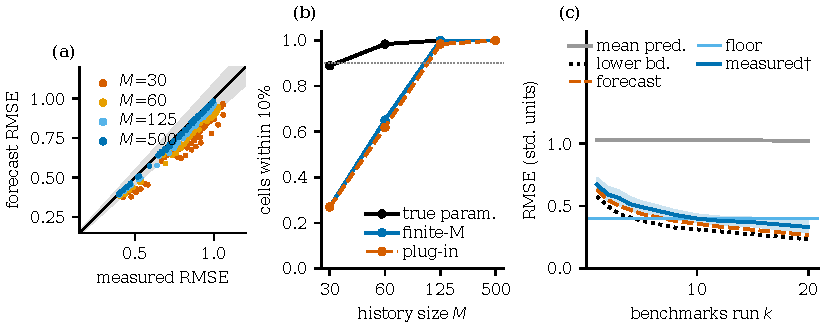
\includegraphics[width=\textwidth]{figures/f2.pdf}
\caption{Forecast against measurement. (a) Synthetic matrices: finite-history forecast against measured RMSE, $\pm10\%$ band, coloured by history size $M$. (b) Share of synthetic cells within 10\% of the measured error for the true parameters, the finite-history forecast and the plug-in forecast. (c) MTEB-A2: the forecast lies below the measured error at every $k$; the grey line is the mean predictor, the lower bound (lower bd.) and the empirical floor are references. The forecast refers to the complement-error greedy$^\dagger$.}
\label{fig:f2}
\end{figure}

\subsection{When selection matters}
Table~\ref{tab:t2} compares selectors and inference methods on the primary family.
With random folds the A-optimal criterion beats random choice at $k=3$ on both MTEB blocks, but not uniformly: on A2 ($N=30$) the gain is not significant at $k=8$ and at $k=20$, two thirds of the benchmarks, it has $52\%$ higher error than random [$+36$, $+72$].
The complement-error greedy$^\dagger$ is better than random at every $k$ of the grid on A1 ($-28$, $-15$, $-15\%$) and A2 ($-20$, $-32$, $-50\%$).
Among the heuristics, pivoted QR, leverage scores and centrality are clearly worse than A-optimal selection on A1 ($-17\%$ to $-61\%$); $k$-medoids clustering is within a few per cent of it and better at $k=20$ on A1 and, markedly, on A2 at $k=8$ and $20$.
A model-free cluster of benchmarks is a strong baseline; the factor model adds the closed-form gain, the forecast, and the target-aware and cost-aware variants of Section~\ref{sec:method}.
In a comparison we added after the pilot and kept outside the declared family, the complement-error greedy$^\dagger$ is never worse than $k$-medoids or forward regression on A1 and A2 but on B it is worse than $k$-medoids at $k=8$ ($+5\%$) and not better than forward regression: simple selectors are competitive there (Appendix~\ref{app:fam}).
On the sparse matrix B (507 models, 598 tasks, 22\% observed; three repetitions) the A-optimal criterion beats random by $22\%$ at $k=3$, ties it at $k=8$ ($-2\%$, not significant) and loses by $14\%$ at $k=20$, where the complement-error greedy$^\dagger$ beats random by $15\%$ and A-optimal by $26\%$ (Appendix~\ref{app:t2full}).
Under folds made of whole organisations, with a bootstrap over organisations (Appendix~\ref{app:fam}), no decision of Table~\ref{tab:t2} changes in the random folds, and the gains at $k=3$ hold on A1 and B ($-27\%$ on A1 and $-12\%$ on B for the complement-error greedy$^\dagger$ against random) and the complement-error greedy stays better than random on A1 at every $k$.
Not all survives: on A2 the gain at $k=3$ does not hold ($-4\%$ for both selectors): one organisation carries most of the error and the A-optimal criterion is no better than random at $k=3$ and $8$ and worse at $k=20$; on B the greedy's gain at $k=20$ is a tie ($+8\%$, n.s.) against $-15\%$.
On the five generative-LLM matrices (five repetitions of family-held-out folds, cluster selection not run; Table~\ref{tab:t3} in Appendix~\ref{app:t2full}) the A-optimal criterion beats random choice at the smallest budgets (HELM Lite $-28\%$ in MSE at $k=2$, HELM MMLU $-25\%$ and the Open LLM Leaderboard subtasks $-23\%$ at $k=3$), and is worse or no better at the largest: $+11\%$ at $k=20$ on HELM MMLU, $+7\%$ at $k=3$ on the six-benchmark Open LLM Leaderboard matrix, no significant difference on LiveBench.
The complement-error greedy$^\dagger$ is never worse than random and is better on HELM Lite, on both Open LLM Leaderboard matrices ($-18\%$ to $-49\%$) and, at $k=3$, on HELM MMLU; on LiveBench (77\% observed) its gain is not significant.

\begin{table}[t]
\centering\scriptsize\setlength{\tabcolsep}{3pt}
\begin{tabular}{@{}lrrr@{}}
\toprule
Comparison & $k=3$ & $k=8$ & $k=20$ \\
\midrule
\multicolumn{4}{@{}l}{\textit{MTEB-A1}} \\
P1 A-optimal vs random & \textbf{$-$28 [$-$33,$-$22]} & \textbf{$-$15 [$-$19,$-$10]} & \textbf{$-$3 [$-$5,$-$2]} \\
P3 A-optimal vs cluster & $+$3 [$-$1,$+$10] & $-$2 [$-$5,$+$1] & \textbf{$+$3 [$+$2,$+$5]} \\
P3 A-optimal vs pivqr & \textbf{$-$42 [$-$48,$-$35]} & \textbf{$-$40 [$-$47,$-$34]} & \textbf{$-$17 [$-$22,$-$12]} \\
P5 FA vs ridge (A-optimal) & 0 [$-$2,$+$2] & $+$2 [$-$1,$+$7] & \textbf{$+$7 [$+$5,$+$9]} \\
P5 FA vs kNN (A-optimal) & $+$9 [$+$2,$+$15] & $+$6 [$-$1,$+$13] & 0 [$-$6,$+$5] \\
P5 FA vs softImpute (A-optimal) & \textbf{$-$21 [$-$28,$-$14]} & \textbf{$-$11 [$-$17,$-$5]} & $+$2 [$-$1,$+$4] \\
P7 complement-error greedy vs A-optimal\,$\dagger$ & 0 & 0 [0,$+$1] & \textbf{$-$12 [$-$16,$-$9]} \\
P7 complement-error greedy vs random\,$\dagger$ & \textbf{$-$28 [$-$33,$-$22]} & \textbf{$-$15 [$-$18,$-$10]} & \textbf{$-$15 [$-$19,$-$12]} \\
\midrule
\multicolumn{4}{@{}l}{\textit{MTEB-A2}} \\
P1 A-optimal vs random & \textbf{$-$20 [$-$25,$-$15]} & $-$3 [$-$9,$+$4] & \textbf{$+$52 [$+$36,$+$72]} \\
P3 A-optimal vs cluster & $+$2 [$-$4,$+$8] & \textbf{$+$16 [$+$8,$+$25]} & \textbf{$+$90 [$+$65,$+$122]} \\
P3 A-optimal vs pivqr & \textbf{$-$23 [$-$34,$-$9]} & $+$17 [$+$2,$+$35] & \textbf{$+$249 [$+$188,$+$324]} \\
P5 FA vs ridge (A-optimal) & 0 [$-$1,$+$1] & \textbf{$+$5 [$+$2,$+$9]} & \textbf{$+$20 [$+$12,$+$31]} \\
P5 FA vs kNN (A-optimal) & \textbf{$+$25 [$+$13,$+$40]} & $+$6 [0,$+$12] & $+$10 [$+$2,$+$18] \\
P5 FA vs softImpute (A-optimal) & \textbf{$-$13 [$-$18,$-$9]} & \textbf{$-$7 [$-$11,$-$2]} & \textbf{$+$11 [$+$7,$+$16]} \\
P7 complement-error greedy vs A-optimal\,$\dagger$ & 0 [$-$3,$+$3] & \textbf{$-$30 [$-$45,$-$17]} & \textbf{$-$67 [$-$88,$-$50]} \\
P7 complement-error greedy vs random\,$\dagger$ & \textbf{$-$20 [$-$24,$-$16]} & \textbf{$-$32 [$-$45,$-$21]} & \textbf{$-$50 [$-$65,$-$37]} \\
\bottomrule
\end{tabular}

\caption{Primary comparisons on MTEB-A1 and A2: relative change in held-out MSE (\%), first named minus second (negative: first is better), with 95\% unadjusted intervals over held-out models; \textbf{bold}: Holm-adjusted $p<0.05$ over the full family of each matrix (P1--P8), of which 8 of the 12 comparisons are shown (the rest: Appendix~\ref{app:t2full}). $\dagger$: added after the pilot. Selectors use factor-posterior inference except where named.}
\label{tab:t2}
\end{table}

\subsection{Groups of tasks and unequal costs}
Two variants of Section~\ref{sec:method} change the question (details and Figure~\ref{fig:f3} in Appendix~\ref{app:groups}).
Choosing benchmarks to predict a group of tasks beats random choice in all ten cells ($12$--$48\%$) but the all-benchmark design in only three ($5$--$12\%$).
Choosing by gain per unit of evaluation time beats the cost-ignorant choice by $44$--$45\%$ on A2 at every budget, where costs are very unequal, but on A1 only at a budget of 5\%.

\subsection{Inference: factor posterior against nonlinear imputers}
Figure~\ref{fig:f6} compares inference methods at the same selected set.
The factor posterior is not the most accurate on MTEB.
At $k=8$ it has $22\%$ (A1) and $25\%$ (A2) higher MSE than ExtraTrees \citep{geurts2006extremely} and $23\%$ (both) than kernel ridge, all Holm-significant; it equals a mixture of factor analysers on A1 ($+0.3\%$) and is $15\%$ worse on A2.
In Table~\ref{tab:t2} it beats softImpute at small $k$ ($-21\%$ at $k=3$ on A1), does not beat ridge or kNN there, and is worse than ridge at $k=20$ on A2 ($+20\%$). On B it beats softImpute at $k=3$ and $8$ ($-22\%$, $-7\%$) and loses to it at $k=20$ ($+10\%$), and is worse than ridge and kNN at every $k$.
On the LLM matrices (Table~\ref{tab:t3}; softImpute not run on the 40-subtask matrix) it beats softImpute everywhere and is indistinguishable from ridge on three of them, but kNN is better on the six-benchmark Open LLM Leaderboard matrix.
What the factor posterior provides in exchange is a predictive variance, hence a forecast of error against $k$ (above), prediction intervals and a stopping rule, which a point-prediction imputer lacks.
The selection gain, however, is not an artefact of the factor model (panels b--d): complement-error selection beats random under all three inference methods at every $k\le20$ on A2 ($-12\%$ to $-51\%$) and under factor analysis and ExtraTrees at every $k\le30$ on A1; under kernel ridge on A1 it helps only at $k=3$ and $8$ and random choice is better at $k=20$ and $30$ ($+17\%$, $+20\%$).
Appendix~\ref{app:rules} compares six inference rules at a fixed selection.

\begin{figure}[t]
\centering
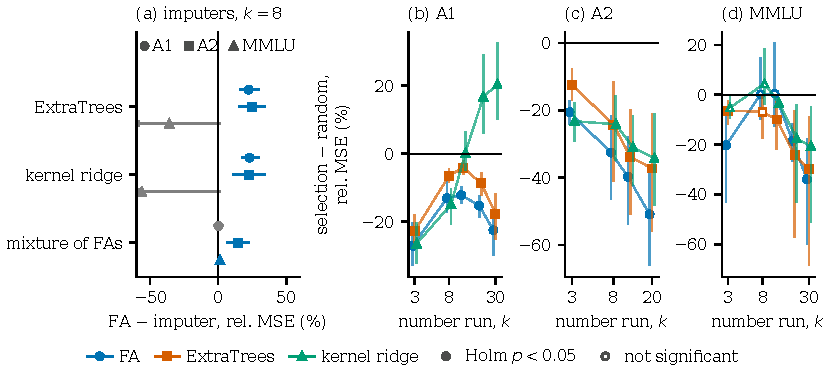
\includegraphics[width=\textwidth]{figures/f6.pdf}
\caption{Inference methods and the selection gain. (a) At the same selected set ($k=8$), FA minus the nonlinear imputer in relative MSE with 95\% intervals; positive means FA is worse; blue: Holm $p<0.05$; arrows: interval cut at the axis. (b--d) A1, A2 and MMLU denote MTEB-A1, MTEB-A2 and HELM MMLU. Complement-error selection minus random choice (relative MSE; negative: selection helps) by inference method; filled: Holm $p<0.05$.}
\label{fig:f6}
\end{figure}

\subsection{Shift}
Under temporal splits (history models are those released earlier) the model-based 90\% intervals cover $0.76$ (A2) and $0.80$ (A1) of the scores on MTEB at $k=3$, and $0.85$ under family-held-out splits; on the LLM matrices coverage is within $0.02$--$0.06$ of nominal (Appendix~\ref{app:shift}).
The error ratio to the mean predictor rises under temporal shift on MTEB (A2 $0.76$ against $0.57$ for random splits), split-conformal coverage stays below $0.90$ ($0.83$, $0.85$), and neither stopping rule is uniformly closer to the measured $k^\ast$.

\subsection{How large must $k$ be?}
We take $k^\ast(\epsilon)$ as the smallest grid $k$ at which the factor-posterior RMSE is at most $\epsilon$ times that of the history-mean predictor, for the complement-error greedy$^\dagger$.
Figure~\ref{fig:f4} places the real matrices on the synthetic grid, whose latent share of variance $h$, history size and spectrum are known.
At $\epsilon=0.7$ one to three benchmarks suffice on every real matrix; at $\epsilon=0.5$ $k^\ast$ is $15$ of $202$ on A1, $5$ of $30$ on A2, $8$ of $40$ on the Open LLM Leaderboard subtasks and $2$ of $57$ on HELM MMLU, while on the sparse matrix B ($h=0.75$) it is not reached within the $20$ benchmarks of the grid (of $598$); the model-based stopping rule would have stopped at $5$ and $3$ on A1 and A2, because its forecast is optimistic.
The latent share alone does not determine $k^\ast$: at $h\approx0.85$ the synthetic $k^\ast$ is $2$ for one factor, $8$--$12$ for four balanced blocks and more than $20$ for a power-law spectrum.
Real matrices with $h$ between $0.75$ and $0.89$ need from $2$ (HELM MMLU) to more than $20$ (B): $k^\ast$ is set by the tolerance and the spectrum, not by $N$.

\begin{figure}[t]
\centering
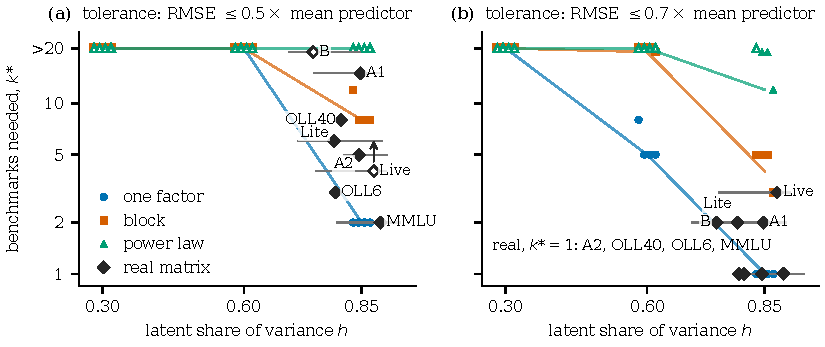
\includegraphics[width=\textwidth]{figures/f4.pdf}
\caption{Benchmarks needed, $k^\ast$, against the latent share of variance $h$. (a) Tolerance: RMSE $\le0.5$ times that of the history-mean predictor; (b) $\le0.7$. Coloured markers: synthetic matrices ($N=48$; one-factor, block and power-law spectra; history sizes $M\in\{30,60,125,500\}$; hollow: not reached by $k=20$), lines: $k^\ast$ from the true parameters. Black diamonds: real matrices at their fitted $h$ (bar: range over folds); hollow: not reached on the grid (arrow where the grid ends below 20). Complement-error greedy$^\dagger$ with factor inference.}
\label{fig:f4}
\end{figure}
